\documentclass{article}
\usepackage[utf8]{inputenc}
\usepackage{amsmath}  
\usepackage{graphicx} % Para incluir imágenes
\usepackage{float}    % Para controlar la ubicación de las imágenes y tablas

\title{Hola, mundo}
\author{Arian Estéfano Gora Ramón}
\date{12 de octubre de 2024}

\begin{document}
	
	\maketitle
	
	\section{Comenzando}
	
	Hola, mundo. Hoy estoy aprendiendo \LaTeX. \LaTeX{} es un excelente lenguaje para producir documentos académicos. Puedo escribir matemáticas en línea, como $a^2 + b^2 = c^2$. También puedo darle a las ecuaciones su propia línea:
	
	\begin{equation}
		\gamma^2 + \theta^2 = \omega^2
	\end{equation}
	
	Las ``ecuaciones de Maxwell'' son nombradas en honor a James Clerk Maxwell y son las siguientes:
	
	\begin{align}
		\nabla \cdot \mathbf{E} &= \frac{\rho}{\varepsilon_0} && \text{Ley de Gauss} \\
		\nabla \cdot \mathbf{B} &= 0 && \text{Ley de Gauss para el magnetismo} \\
		\nabla \times \mathbf{E} &= - \frac{\partial \mathbf{B}}{\partial t} && \text{Ley de Faraday} \\
		\nabla \times \mathbf{B} &= \mu_0 \left( \mathbf{J} + \varepsilon_0 \frac{\partial \mathbf{E}}{\partial t} \right) && \text{Ley de Ampere}
	\end{align}
	
	Las ecuaciones (2), (3), (4) y (5) son algunas de las más importantes en Física.
	
	\section{¿Qué hay sobre las ecuaciones matriciales?}
	
	\begin{equation}
		\begin{pmatrix}
			a_{11} & a_{12} & \dots  & a_{1n} \\
			a_{21} & a_{22} & \dots  & a_{2n} \\
			\vdots & \vdots & \ddots & \vdots \\
			a_{m1} & a_{m2} & \dots  & a_{mn}
		\end{pmatrix}
		\begin{pmatrix}
			x_1 \\
			x_2 \\
			\vdots \\
			x_n
		\end{pmatrix}
		=
		\begin{pmatrix}
			w_1 \\
			w_2 \\
			\vdots \\
			w_m
		\end{pmatrix}
	\end{equation}
	
	\section{Tablas y Figuras}
	
	Crear una tabla no es muy diferente de crear una matriz:
	
	\begin{table}[H]
		\centering
		\begin{tabular}{|c|c|c|c|}
			\hline
			$x$ & 1 & 2 & 3 \\
			\hline
			$f(x)$ & 4 & 8 & 12 \\
			\hline
		\end{tabular}
		\caption{Mi primera tabla.}
	\end{table}
	
	Para insertar una imagen, uso el siguiente comando:
	
	\begin{figure}[H]
		\centering
		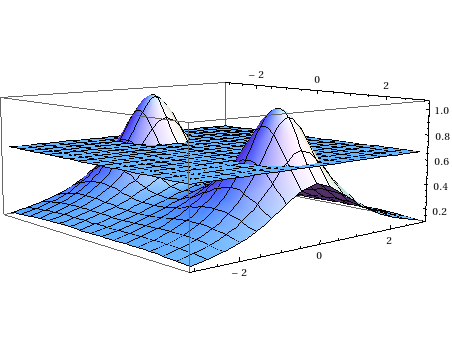
\includegraphics[width=0.5\textwidth]{image.png}
		\caption{Cualquier imagen.}
	\end{figure}
	
	
\end{document}
